\documentclass[conference]{IEEEtran}

\usepackage[utf8]{inputenc}
\usepackage[T1]{fontenc}
\usepackage{silence}\WarningsOff[latexfont]

\usepackage{amsmath}

\RequirePackage{tikz}[2010/10/13]
\usetikzlibrary{arrows,automata,calc,intersections,patterns,decorations.pathmorphing,decorations.pathreplacing}

\usepackage{graphicx}
\usepackage{cite}
\usepackage{url}
\usepackage[caption=false,font=footnotesize]{subfig}
\usepackage[binary-units,per-mode=symbol]{siunitx}
\sisetup{list-final-separator = {, and }}
\usepackage{booktabs}
\usepackage{pifont}
\usepackage{microtype}
\usepackage{textcomp}
\usepackage[american]{babel}
\usepackage[noabbrev,capitalise]{cleveref}
\usepackage{xspace}
\usepackage{hyphenat}
\usepackage[draft,inline,nomargin,index]{fixme}
\fxsetup{theme=color}
\usepackage{grffile}
\usepackage{xfrac}
\usepackage{multirow}
\RequirePackage{xstring}
\RequirePackage{xparse}
\RequirePackage[index=true]{acro}

\NewDocumentCommand\acrodef{mO{#1}mG{}}{\DeclareAcronym{#1}{short={#2}, long={#3}, #4}}
\NewDocumentCommand\acused{m}{\acuse{#1}}

\usepackage{upquote}

\acrodef{DES}{Discrete Event Simulation}
\acrodef{MAC}{Medium Access Control}

\begin{document}

\title{Python Simulator Extension}
\author{
	\IEEEauthorblockN{Davide Pedranz, Mat. number 189295}
	\texttt{davide.pedranz@studenti.unitn.it}
}

\maketitle

\begin{abstract}
Simulators are powerful tools to analyze the performances of a system.
They can be used to evaluate a system before building it, compare different design choices and validate models.
In this assignment, starting from a discrete event simulator for the Aloha MAC protocol, we will implement simulators some variations of the protocol and evaluate the performances as a function of the load offered to the network.
\end{abstract}

\acresetall

\section{Introduction}
\label{sec:introduction}

\ac{DES} is a powerful and widely used technique to analyze, compare and evaluate the performances of a system.
Performance evaluation is fundamental to take the right decisions in the design and construction of a system and guarantee that it behaves as expected.  

In this assignment, we will start from a Python simulator for the Aloha \ac{MAC} protocol to implement some variations of it.
We will briefly discuss the standard behaviour of Aloha and how the protocol is implemented in the original simulator.
We will introduce, one at a time, the modifications to the protocol and describe the respective implementations.
Finally, we will compare their performances using the results of the simulations.

\section{Aloha}
\label{sec:aloha}

A \ac{MAC} protocol defines how stations access a shared channel in order to transmit messages to the others.
Aloha is a very simple \ac{MAC} protocol developed by Norman Abramson and colleagues at the University of Hawaii in the 1970s to realize a broadcasting communication between nodes spread on different islands in the archipelago. 

The behaviour of the original Aloha is the following: when a packet arrives to the station, it is immediately transmitted to all stations in the communication range.
When idle, the station listens for variations of energy in the channel in order to be able to detect and receive incoming packets.
After transmitting or receiving a packet, a small amount of time is required to process it.
If new packets arrive while the station is already transmitting, receiving or processing a packet, they are queued and will be transmitted as soon as the station finishes the current action.
If multiple packets are transmitted at the same time, they are very likely to collide and be corrupted.

Aloha does not try to avoid or detect collisions.
In case of collisions, the packet are not recognizable and thus simple discarded.
In other words, there is no guarantee that a packet is correctly received by the other stations.

\section{Original Simulator}
\label{sec:simulator_aloha}

The simulator is event driven and implemented in plain Python.
Events are stored in a priority queue, where the priority is given by the timestamp of the event.
The simulator loops over the events queue, until the wanted simulation time is reached.
At each iteration, the first event is extracted from the queue and precessed.
Each step can change the internal state of the simulator, schedule new events and generate logs, which are collected in a log file.
The produced logs are used to compute metrics that can be used to evaluate the overall performances of the simulated system.

\begin{figure}[h]
	\centering
	\includegraphics[width=0.88\columnwidth]{figures/states/aloha}
	\caption{State machine for a single station for Aloha. Stations can be in $4$ different states, represented by the circles. Arrows indicate the transitions from one state to the other on a given event.}
	\label{fig:aloha_states}
\end{figure}

\cref{fig:aloha_states} shows the possible states of a station:

\begin{itemize}
    \item \textbf{IDLE} - the station is not doing anything,
    \item \textbf{RX} - the station is receiving a packet,
    \item \textbf{TX} - the station is transmitting a packet,
    \item \textbf{PROC} - the station is processing the last packet.
\end{itemize}

The behaviour of a station is determined by its state, the packets that are currently being received (\texttt{recv\_count}) and the length of its queue.
If multiple packets arrive at the same time, they collide and the simulator marks them as corrupted.

Each packet need some time to be propagated through the channel and some other time to be received from a station, depending on the packet size.
The size of the packets and their interarrival time are computed using random values taken from some distribution.
The distributions and their parameters can be configured in the configuration file.

The events used in the simulator are:

\begin{itemize}
    \item \textbf{arrival} - a new packet to transmit arrives to the station,
    \item \textbf{start\_rx} - the station starts to receive a packet,
    \item \textbf{end\_rx} - the station finishes to receive a packet,
    \item \textbf{end\_tx} - the station finished to transmit a packet,
    \item \textbf{end\_proc} - the station finished to process a packet,
    \item \textbf{rx\_timeout} - the maximum time allowed to receive the packet is over, the packet is probably corrupted and must be discarded.
\end{itemize}

The simulator schedules the first packet arrival on each node.
Packets are transmitted to all reachable nodes: the channel object compute the nodes to send the packet to and schedules, after some propagation time, an arrival on the receivers.

\section{Realistic Propagation}
\label{sec:realistic_propagation}

The first implemented change is the packets' propagation model.
The original simulator uses a disk model: a packet is always correctly received from all and only the stations in the range of the transmitter if no collision occur.
More formally, the receiving probability for a packet is modelled as follows:

\begin{equation}
Pr(correct\ |\ d) =
    \left\{
    	\begin{array}{ll}
    		1 & \mbox{if } d < RX_{range} \\
    		0 & \mbox{otherwise}
    	\end{array}
    \right.
    \label{eq:original}
\end{equation}

In the real world, however, signals soften with the distance.
A simple model of this phenomena is the following:

\begin{equation}
Pr(correct\ |\ d) =
    \left\{
    	\begin{array}{ll}
    		1 - \frac{d}{RX_{range}} & \mbox{if } d < RX_{range} \\
    		0 & \mbox{otherwise}
    	\end{array}
    \right.
    \label{eq:realistic}
\end{equation}

It is possible to specify the model to use in the simulator using the \texttt{propagation} parameter in the configuration file.
Allowed values are \texttt{original} for the model of \cref{eq:original} or \texttt{realistic} for the model of \cref{eq:realistic}.

If the realistic model is selected, the channel tags each packet with the probability of correct receiving for the receiver.
When a node processes a not corrupted packet, a random variable from a Uniform distribution between $0$ and $1$ is extracted: if the value is higher or equal to the probability of correct receiving, the packet is marked as correctly received, otherwise it is marked as corrupted.
The simulator distinguish between ``corrupted for a collision'' and ``corrupted because of the distance'' to allow a detailed analysis of the results.

\section{Trivial Carrier Sensing}
\label{sec:trivial}

Trivial Carrier Sensing extends the Aloha protocol described in \cref{sec:aloha} to include a carrier sensing function that tries to avoid collisions between packets.
Before sending a packet, the station listens the energy on the channel to detect possible incoming packets.
If the channel is free, the packet is transmitted immediately.
If the channel is occupied, the transmission is delayed to when the channel becomes free.

The simulator assumes that a station can correctly determine if the channel is free or not with a probability of $1$.
The station can either sense the channel, transmit, receive or process a packet at a time.
It is not possible, for instance, to sense the channel when transmitting a packet.
We assume that the station can sense the channel instantly.

Carrier sensing is introduced on end\_proc events: if the channel is not free, the node move to the new state \textbf{WC} (WAITING\_FREE\_CHANNEL) and waits until the channel is free.
When the channel gets free (end\_rx with recv\_count = 0), it moves to TX and transmit the next packet if any, otherwise to IDLE.
As a side effect, it is not possible anymore to get the events for start and end receiving in the IDLE state, since they are captured from the WC state.
\cref{fig:trivial_cs_states} shows the state machine diagram for the Trivial Carrier Sensing protocol.

\begin{figure}[h]
	\centering
	\includegraphics[width=0.95\columnwidth]{figures/states/trivial}
	\caption{State machine for a single station for Trivial Carrier Sensing.}
	\label{fig:trivial_cs_states}
\end{figure}

\section{Simple Carrier Sensing}
\label{sec:simple}

Simple Carrier Sensing tries to avoid collisions on the channel using a p-persistent approach.
When a station wants to transmit, it checks if the channel is free or occupied.
In the first case, it transmit immediately.
In the second case, it re-schedules the transmission with persistence $p$. $p$ is a probability that defines if the transmission is scheduled immediately after the channel becomes free or postponed of an exponential random time with average $T_r = 10T_t$, where $T_t$ is the time needed to transmit the maximum size packet.

We assume that the scheduled transmissions are cancelled if some packets arrive in the meanwhile.
After the new packet is received and processed, the postponed packet can be eventually transmitted: a new random variable is used to decide whether the packet should be transmitted immediately of postponed again.

\begin{figure}[ht]
	\centering
	\includegraphics[width=\columnwidth]{figures/states/simple}
	\caption{State machine for a single station for Simple Carrier Sensing.}
	\label{fig:simple_cs_states}
\end{figure}

\cref{fig:trivial_cs_states} shows the state machine diagram for the Simple Carrier Sensing.
The event \textbf{wt\_timeout} indicate the scheduled transmission of a packet.
The new state \textbf{WT} (WAITING\_TO\_TRANSMIT) indicate that the station is idle but waiting to transmit a rescheduled packet.

\section{Simulations}
\label{sec:simulation}

The simulator models the interarrival time between packets to transmit to a station with an exponential distribution.
The size of each packet is extracted from a uniform distribution between $32$ and $1460 B$.
Each station has a limited amount of memory, so it can store at most $2$ packets in a queue.
Packets that do not fit in the queue are discarded.
All simulations use the same network topology, shown in \cref{fig:network}.
Each simulation is run with multiple seeds for the pseudonumber generator in order to get more robust results.

\begin{figure}[ht]
	\centering
	\includegraphics[width=0.9\columnwidth]{figures/plots/topology}
	\caption{The plot show the topology of the network used to run all simulations. Only nodes connected by a dashed line can communicated with each other.}
	\label{fig:network}
\end{figure}

\section{Metrics}
\label{sec:metrics}

\subsection{Offered load}
The total offered load is computed as the sum of the offered load from all stations, expressed in $Mbps$.
Formally, we have:

\begin{equation}
    load = \sum_{\substack{s \in stations \\ p \in packets(s)}} \frac{size(p)}{1024 ^ 2},
    \label{eq:throughput_raw}
\end{equation}

where $packets(s)$ denotes the packets generated by station $s$ for in \SI{1}{\second} of time and $size(p)$ is the dimension of packet $p$ in \si{\byte}.
Since the distributions $size(p) \sim X$ and $interarrival \,\, time \sim Y$ are respectively uniform and exponential

\begin{equation*}
    f_X(x) =
    \begin{cases}
        \frac{1}{1460-32} & \text{if $x \in [32, 1460]$}\\[0.3em]
        0 & \text{otherwise}
    \end{cases},
\end{equation*}
\begin{equation*}
    f_Y(y) = \lambda e^{-\lambda y},
\end{equation*}

and for each simulation we have a big number of generated packets, we can simplify \cref{eq:throughput_raw} to the following formula:

\begin{equation*}
    load \, [\si{Mbps}] = \lambda |stations| \frac{32+1460}{2} \frac{8}{1024 ^ 2},
\end{equation*}

which allows a more efficient computation of the metrics.


\subsection{Throughput}
The throughput at the receiver is defined as the amount of correctly received information over the simulation time:

\begin{equation}
    throughput \, [\si{Mbps}] = \frac{\sum_{p \in correct\_packets} size(p) \frac{8}{1024^2}}{simulation\_time} .
\end{equation}


\subsection{Collision Rate}
The collision rate measure the amount of packets that do not reach correctly the destination due to collisions on the channel:

\begin{equation}
    collision\_rate = \frac{|corrupted|}{|transmitted|},
\end{equation}

where $corrupted$ indicate the set of packets which where corrupted due to collisions and $transmitted$ denote the set of all sent packets.


\subsection{Packet Drop Rate}
The drop rate measure the amount of packets that where discarded by the stations because the queue of packets to transmit was already full.
Formally:

\begin{equation}
    drop\_rate = \frac{|dropped|}{|generated|},
\end{equation}

where $dropped$ is the set of packets dropped by a station and $generated$ denote the set of packets generated.
Note that $generated$ is different from $transmitted$, since the first includes also the packets dropped without sending them.


\subsection{Channel Corruption Rate}
The channel corruption rate measure the amount of packets that are corrupted by the channel before reaching the destination. Collisions are not considered for this metric.
We define the channel corruption rate as:

\begin{equation}
    corruption\_rate = \frac{|corrupted|}{|generated|},
\end{equation}

where $corrupted$ is the set of packets corrupted by the channel and $generated$ denote the set of packets generated.

\section{Performances}
\label{sec:performances}

\begin{figure}[t!]
	\centering
	\centering
	\includegraphics[width=\columnwidth]{figures/plots/realistic_tr}
	\caption{Throughput of the different protocols in respect to the total load on the channel with the realistic propagation model. Simple Carrier Sensing performs better then Trivial Carrier Sensing and Aloha. The highest throughput is obtained at \SI{10}{Mbps} of load. When the load is higher, the performances of all protocols tend to zero.}
	\label{fig:tr}
\end{figure}

\begin{figure}[t!]
	\centering
    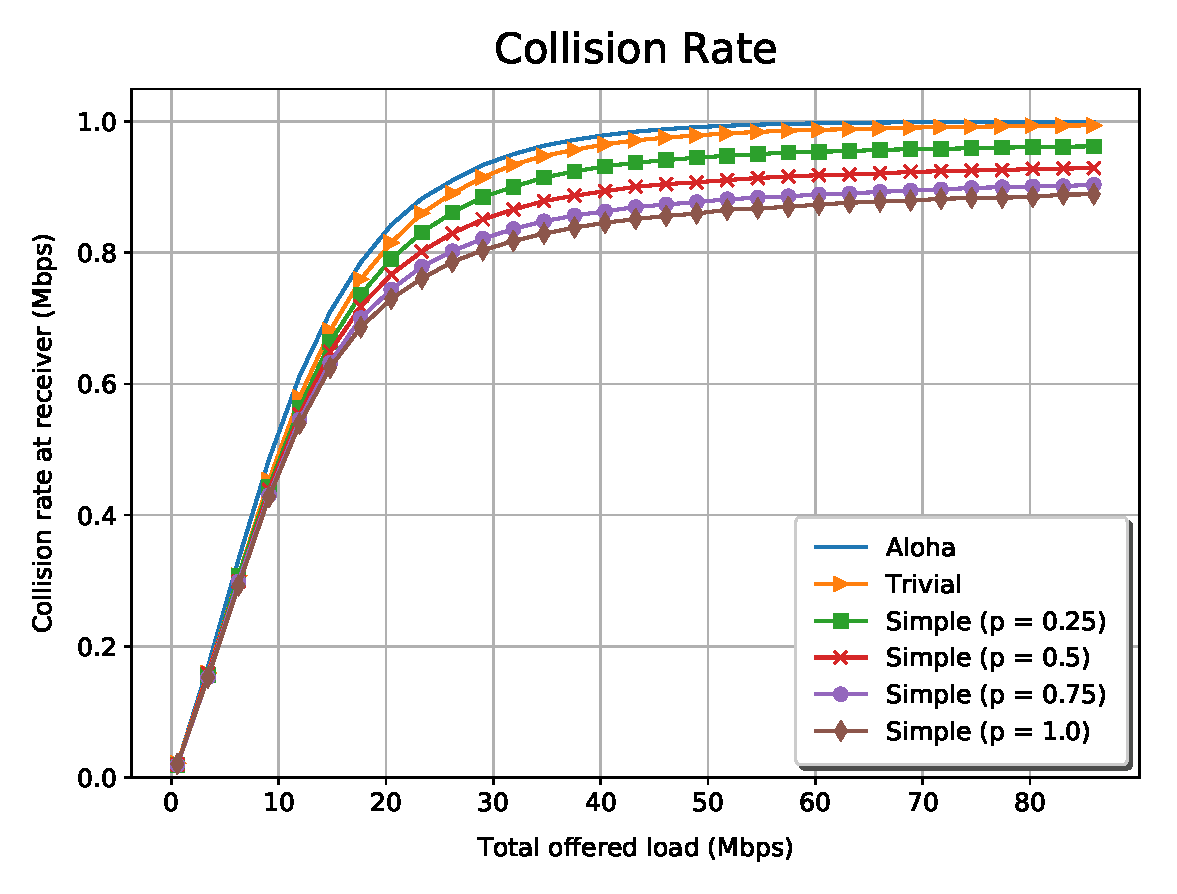
\includegraphics[width=\columnwidth]{figures/plots/realistic_cr}
	\caption{Collision Rate of the different simulations with respect to the total offered load. High collision rates degrade the performances of the protocol. Aloha and Trivial Carrier Sensing have the higher collision rate.}
	\label{fig:cr}
\end{figure}

\begin{figure}[t!]
	\centering
    \includegraphics[width=\columnwidth]{figures/plots/realistic_dr}
	\caption{Packet Drop Rate at the sender for the realistic propagation model. Aloha has a packet drop rate significantly lower then the other protocols, while there is not big difference between Simple and Trivial Carrier Sensing.}
	\label{fig:dr}
\end{figure}

\begin{figure}[t!]
	\centering
    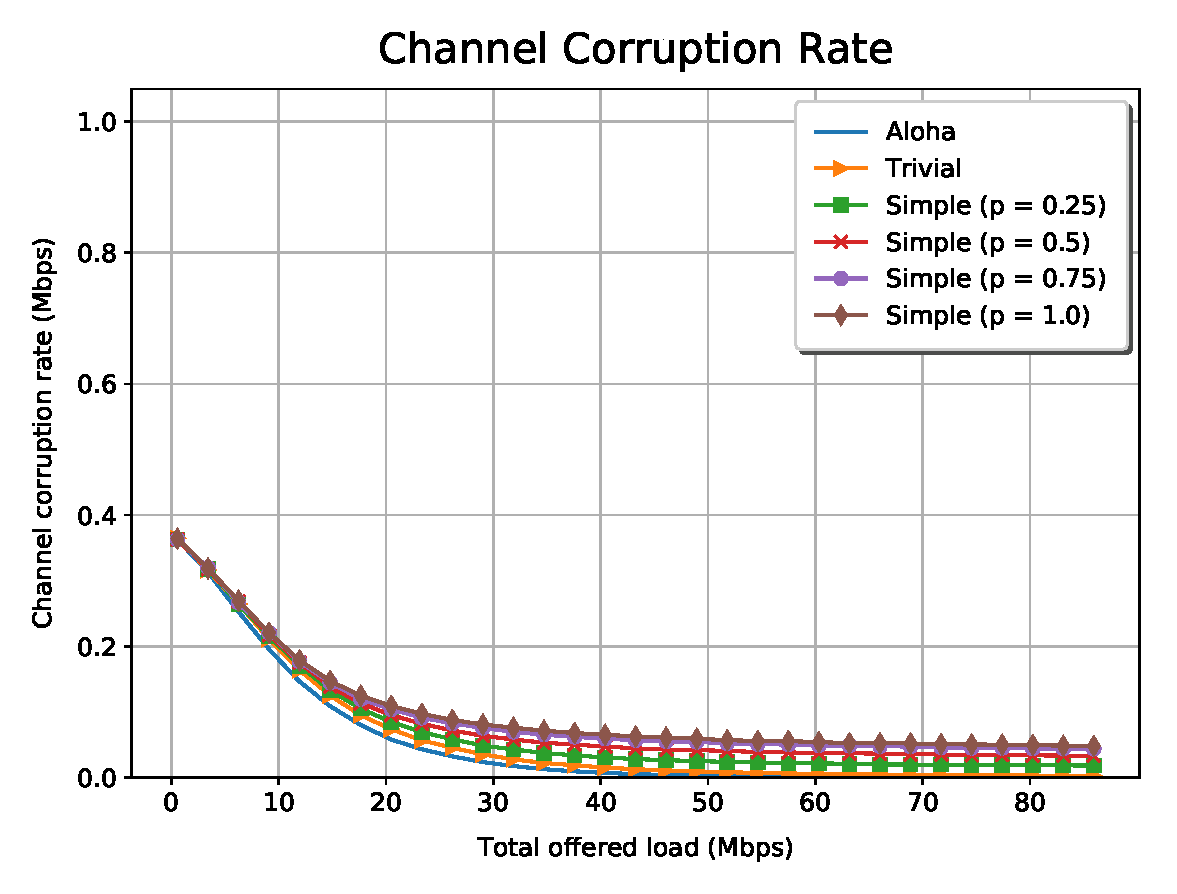
\includegraphics[width=\columnwidth]{figures/plots/realistic_cc}
	\caption{Channel Corruption Rate of the different simulations with respect to the total load on the channel. With high loads, the packets propagation model becomes less important.}
	\label{fig:cc}
\end{figure}


In this section, we compare the different variants of the protocol.
Unless otherwise specified, the results refer to the realistic propagation model.

\subsection{Protocol}
\cref{fig:tr} show that Simple Carrier Sensing performed better then Trivial Carrier Sensing, which performed better than Aloha in terms of throughput.
The increase in throughput is related to the reduction of collisions: indeed, it is easy to see in \cref{fig:cr}  that collision rate of Aloha saturates and Trivial Carrier Sensing tends to \num{1} much quicker than Simple Carrier Sensing.
Simple Carrier Sensing strategy to avoid collisions seems to be more effective then the Trivial one, which in turn is better then Aloha.
In particular, the strategy of Trivial Carrier Sensing is not effective, since all stations will start to transmit together as soon as the channel is free.
The random nature of Simple Carrier Sensing helps to reduce this effect.
The packet drop rate metric confirm this statement: Simple Carrier Sensing has a higher drop rate, which indicate a higher average waiting time to transmit a packet.
When the channel is saturated, most packets are dropped at the sender.


This phenomena is confirmed by the drop rate metric showed in \cref{fig:dr}.
Aloha never senses the channel before transmitting, thus its drop rate increases much slower then Trivial and Simple Carrier Sensing.
On the contrary, with high loads the channel is saturated and most stations are stuck waiting for the channel to be free: most packets are do not fit the limited queue of the stations and are dropped at the sender.

It is interesting to observe the channel corruption rate, showed in \cref{fig:cc}.
With high loads, only a smaller percentage of the packets is corrupted because of the realistic propagation model used.
Most packets are corrupted by collisions.


\subsection{Persistence}
The behaviour of Simple Carrier Sensing is highly dependent of the parameter $p$ used for the persistence.
When $p$ tends to \num{1}, Simple Carrier Sensing behaves exactly like Trivial Carrier Sensing.
When $p$ tends to \num{0}, Simple Carrier Sensing will always wait a random exponential time before transmitting a packet if the channel is occupied.
For intermediate values of $p$, the behaviour is a mixture.
\cref{fig:tr} shows the throughput for different values of $p$: with the given network, higher values of $p$ correspond to a higher throughput.


\subsection{Propagation Model}
The propagation model does not influence the performances of the protocols with respect to the original Aloha.
In fact, the simulations run with the realistic propagation model show exactly the same results as the realistic model.
The throughput for the disk model is about the double of the realistic model.

\section{Conclusion}
\label{sec:conclusion}

In this work, we built a simulator for a simple \ac{MAC} protocol and analyzed the performances of some variants of Aloha.
We started with a description of the original simulator for Aloha.
Then, we described the modifications done to implement the realistic propagation model (\cref{sec:realistic_propagation}), Trivial Carrier Sensing and Simple Carrier Sensing.
Finally, we compared the performances of the different protocols for both propagation models and different traffic loads.

According to the run simulations, Aloha is the worst protocol among the analyzed ones.
Trivial Carrier Sensing is slightly better than Aloha, but has still problems with high loads on the channel.
Simple Carrier Sensing achieved considerably better performances then Trivial Carrier Sensing, most probably for its random nature that breaks the synchronicity between different stations.
Among the possible values for the persistence, $p = \num{0}$ seems to be the best choice.
No protocol can handle high load on the network: in fact, the throughput decreases at about \SI{10}{Mbps} of load.
The same results are valid for the original propagation model.


% \bibliographystyle{IEEEtran}
% \bibliography{references}

\end{document}
